\documentclass{article}

\usepackage[utf8]{inputenc}
\usepackage{graphicx}
\usepackage{amsmath}
\usepackage[letterpaper, portrait, margin=1in]{geometry}
\usepackage{booktabs}

\title{Biomaterials HW 6}
\author{Nikhil Menon}
\date{October 19th, 2016}

\begin{document}

\maketitle

1. Initially, the instantaneous copolymer compositions can be calculated using the formula
$$F_A=\frac{r_Af_A^2+f_Af_B}{r_Af_A^2+2f_Af_B+r_Bf_B^2}$$

At 10\% conversion, 
$$f_A=\frac{60}{40+60}=0.6,f_B=0.4,F_A=0.2308$$

Assuming there are a total of 10 mol of starting material, we can calculate the mols of A consumed as
$$0.2308*10 mol*10=0.2308 mol$$

Thus, the new monomer composition is
$$f_1=\frac{6-0.2308}{10-1}=0.641$$

The new copolymer composition can be calculated from this number, and the average copolymer composition is $$\frac{0.2308 mol}{1 mol}=0.2308$$

The remaining numbers can be calculated in a similar way and are shown below.


\begin{tabular}{*4l}    \toprule
\emph{\% Conversion} & \emph{Monomer Composition} & \emph{Copolymer Composition} & \emph{Cumulative Copolymer Composition} \\
\midrule
10\% & 0.6 & 0.2308 & 0.2308\\ 
20\% & 0.6410 & 0.2632 & 0.2470\\
30\% & 0.6883 & 0.3063 & 0.2667\\
40\% & 0.7428 & 0.3662 & 0.2916\\
50\% & 0.8056 & 0.4532 & 0.3239\\
60\% & 0.8761 & 0.5857 & 0.3676\\
70\% & 0.9487 & 0.7871 & 0.4275\\
80\% & 1 & 1 & 0.5007\\
90\% & 1 & 1 & 0.5547\\
100\% & 1 & 1 & 0.6032\\
\bottomrule
\end{tabular}

Below, blue represent monomer composition, red represents copolymer composition, and yellow represents cumulative copolymer composition
\begin{figure}[h]
\centering
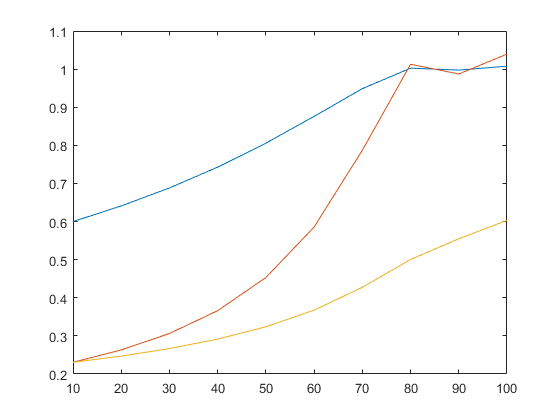
\includegraphics[scale=0.6]{P1.png}
\end{figure}
\vspace{1in}

\section*{2A. Vinyl Chloride}
a. At equimolar concentrations, $f_a=f_b=0.5, r_A=0.23, r_B=1.68$. Therefore,
$$F_A=\frac{r_Af_A^2+f_Af_B}{r_Af_A^2+2f_Af_B+r_Bf_B^2}=0.31$$
b. If $F_A=0.5$, we can reverse-solve for $f_A$ using the formula above after substituting $f_B=1-f_A$ to get $$0.5=\frac{r_Af_A^2+f_A(1-f_A)}{r_Af_A^2+2f_A(1-f_A)+r_B(1-f_A)^2}=\frac{(r_A-1)f_A^2+f_A}{(r_A+r_B-2)f_A^2+(2-2r_B)f_A+r_B}$$
Therefore, 
$$ f_A=0.73, \frac{[A]}{[B]}=\frac{f_A}{1-f_A}=2.70$$

\section*{2B. Acrylonitrile}
a. At equimolar concentrations, $f_a=f_b=0.5, r_A=0.06, r_B=4.05$. Therefore,
$$F_A=\frac{r_Af_A^2+f_Af_B}{r_Af_A^2+2f_Af_B+r_Bf_B^2}=0.17$$
b. Using the same method above, we get that $$f_A=0.89, \frac{[A]}{[B]}=8.09$$

\section*{2C. Styrene}
a. At equimolar concentrations, $f_a=f_b=0.5, r_A=0.01, r_B=55$. Therefore,
$$F_A=\frac{r_Af_A^2+f_Af_B}{r_Af_A^2+2f_Af_B+r_Bf_B^2}=0.018$$
b. Using the same method above, we get that $$f_A=0.98, \frac{[A]}{[B]}=49$$
\end{document}